%%%%%%%%%%%%%%%%%%%%%%%%%%%%%%%%%%%%%%%%%%%%%%%%%%%%%%%%%%%%%%%%%%%%
%%%%%%%%%%%%%%%%%%%%%%%%%%%%%%%%%%%%%%%%%%%%%%%%%%%%%%%%%%%%%%%%%%%%
%%                                                                %%
%% An example for writting your thesis using LaTeX                %%
%% Original version by Luis Costa,  changes by Perttu Puska       %%
%% Support for Swedish added 15092014                             %%
%%                                                                %%
%% This example consists of the files                             %%
%%         thesistemplate.tex (versio 2.01)                       %%
%%         opinnaytepohja.tex (versio 2.01) (for text in Finnish) %%
%%         aaltothesis.cls (versio 2.01)                          %%
%%         kuva1.eps                                              %%
%%         kuva2.eps                                              %%
%%         kuva1.pdf                                              %%
%%         kuva2.pdf                                              %%
%%                                                                %%
%%                                                                %%
%% Typeset either with                                            %%
%% latex:                                                         %%
%%             $ latex opinnaytepohja                             %%
%%             $ latex opinnaytepohja                             %%
%%                                                                %%
%%   Result is the file opinnayte.dvi, which                      %%
%%   is converted to ps format as follows:                        %%
%%                                                                %%
%%             $ dvips opinnaytepohja -o                          %%
%%                                                                %%
%%   and then to pdf as follows:                                  %%
%%                                                                %%
%%             $ ps2pdf opinnaytepohja.ps                         %%
%%                                                                %%
%% Or                                                             %%
%% pdflatex:                                                      %%
%%             $ pdflatex opinnaytepohja                          %%
%%             $ pdflatex opinnaytepohja                          %%
%%                                                                %%
%%   Result is the file opinnaytepohja.pdf                        %%
%%                                                                %%
%% Explanatory comments in this example begin with                %%
%% the characters %%, and changes that the user can make          %%
%% with the character %                                           %%
%%                                                                %%
%%%%%%%%%%%%%%%%%%%%%%%%%%%%%%%%%%%%%%%%%%%%%%%%%%%%%%%%%%%%%%%%%%%%
%%%%%%%%%%%%%%%%%%%%%%%%%%%%%%%%%%%%%%%%%%%%%%%%%%%%%%%%%%%%%%%%%%%%

%% Uncomment one of these:
%% the 1st when using pdflatex, which directly typesets your document in
%% pdf (use jpg or pdf figures), or
%% the 2nd when producing a ps file (use eps figures, don't use ps figures!).
\documentclass[english,12pt,a4paper,pdftex,sci,utf8]{aaltothesis}
%\documentclass[english,12pt,a4paper,dvips]{aaltothesis}

%% To the \documentclass above
%% specify your school: arts, biz, chem, elec, eng, sci
%% specify the character encoding scheme used by your editor: utf8, latin1

%% Use one of these if you write in Finnish (see the Finnish template):
%%
%\documentclass[finnish,12pt,a4paper,pdftex,elec,utf8]{aaltothesis}
%\documentclass[finnish,12pt,a4paper,dvips]{aaltothesis}

\usepackage{graphicx}
\usepackage{epstopdf}

%% Use this if you write hard core mathematics, these are usually needed
\usepackage{amsfonts,amssymb,amsbsy,amsmath}

%% Use the macros in this package to change how the hyperref package below 
%% typesets its hypertext -- hyperlink colour, font, etc. See the package
%% documentation. It also defines the \url macro, so use the package when 
%% not using the hyperref package.
%%
%\usepackage{url}

%% Use this if you want to get links and nice output. Works well with pdflatex.
\usepackage{hyperref}
\hypersetup{pdfpagemode=UseNone, pdfstartview=FitH,
  colorlinks=true,urlcolor=red,linkcolor=blue,citecolor=black,
  pdftitle={Default Title, Modify},pdfauthor={Your Name},
  pdfkeywords={Modify keywords}}


%% All that is printed on paper starts here
\begin{document}

%% Change the school field to specify your school if the automatically 
%% set name is wrong
% \university{aalto-yliopisto}
% \university{aalto University}
% \school{Sähkötekniikan korkeakoulu}
\school{School of Science}

%% Only for B.Sc. thesis: Choose your degree programme. 
\degreeprogram{Mathematics and Systems Analysis}
%%

%% ONLY FOR M.Sc. AND LICENTIATE THESIS: Specify your department,
%% professorship and professorship code. 
%%
%\department{Department of Radio Science and Technology}
%\professorship{Circuit theory}
%%

%% Valitse yksi näistä kolmesta
%%
%% Choose one of these:
\univdegree{BSc}
%\univdegree{MSc}
%\univdegree{Lic}

%% Your own name (should be self explanatory...)
\author{Pasi Pyrrö}

%% Your thesis title comes here and again before a possible abstract in
%% Finnish or Swedish . If the title is very long and latex does an
%% unsatisfactory job of breaking the lines, you will have to force a
%% linebreak with the \\ control character. 
%% Do not hyphenate titles.
%% 
\thesistitle{Lattice Codes and Sphere Decoding}

\place{Espoo}

%% For B.Sc. thesis use the date when you present your thesis. 
%% 
%% Kandidaatintyön päivämäärä on sen esityspäivämäärä! 
\date{10.7.2017}

%% B.Sc. or M.Sc. thesis supervisor 
%% Note the "\" after the comma. This forces the following space to be 
%% a normal interword space, not the space that starts a new sentence. 
%% This is done because the fullstop isn't the end of the sentence that
%% should be followed by a slightly longer space but is to be followed
%% by a regular space.
%%
\supervisor{Prof.\ Camilla Hollanti} %{Prof.\ Pirjo Professori}

%% B.Sc. or M.Sc. thesis advisors(s). You can give upto two advisors in
%% this template. Check with your supervisor how many official advisors
%% you can have.
%%
%\advisor{Prof.\ Pirjo Professori}
\advisor{Prof.\ Marcus Greferath}
\advisor{D.Sc.\ Oliver Gnilke}
%\advisor{M.Sc.\ Polli Pohjaaja}

%% Aalto logo: syntax:
%% \uselogo{aaltoRed|aaltoBlue|aaltoYellow|aaltoGray|aaltoGrayScale}{?|!|''}
%%
%% Logo language is set to be the same as the document language.
%% Logon kieli on sama kuin dokumentin kieli
%%
\uselogo{aaltoRed}{''}

%% Create the coverpage
%%
\makecoverpage


%% Note that when writting your master's thesis in English, place
%% the English abstract first followed by the possible Finnish abstract

%% English abstract.
%% All the information required in the abstract (your name, thesis title, etc.)
%% is used as specified above.
%% Specify keywords
%%
%% Kaikki tiivistelmässä tarvittava tieto (nimesi, työnnimi, jne.) käytetään
%% niin kuin se on yllä määritelty.
%% Avainsanat
%%
\keywords{sphere decoding, space--time lattice codes, wireless communications}
%% Abstract text
\begin{abstractpage}[english]
 \end{abstractpage}

%% Force a new page so that the possible English abstract starts on a new page
%%
%% Pakotetaan uusi sivu varmuuden vuoksi, jotta 
%% mahdollinen suomenkielinen ja englanninkielinen tiivistelmä
%% eivät tule vahingossakaan samalle sivulle

\newpage

%% Preface
%%
%% Esipuhe 
%\mysection{Preface}


%\vspace{5cm}
%Otaniemi, 16.1.2015

%\vspace{5mm}
%{\hfill Pasi Pyrrö \hspace{1cm}}

%% Force new page after preface
%\newpage


%% Table of contents.
\thesistableofcontents


%% Symbols and abbreviations
\mysection{Symbols and abbreviations}

\subsection*{Symbols}

\begin{tabular}{ll}
$\mathbb{Z}$  & Set of integers \\
$\mathbb{C}$  & Field of complex numbers \\
$\mathbf{x}$  & Vector \\
$\mathbf{X}$  & Matrix \\
\end{tabular}

\subsection*{Operators}

\begin{tabular}{ll}
$\| \cdot \| $     & Euclidean norm \\
det$(\mathbf{X})$  & Determinant of matrix $\mathbf{X}$
\end{tabular}

\subsection*{Abbreviations}

\begin{tabular}{ll}
SNR & Signal to noise ratio \\
CVP & Closest vector problem \\
MIMO & Multiple input multiple output
\end{tabular}


%% Tweaks the page numbering to meet the requirement of the thesis format:
%% Begin the pagenumbering in Arabian numerals (and leave the first page
%% of the text body empty, see \thispagestyle{empty} below).
%% Additionally, force the actual text to begin on a new page with the 
%% \clearpage command.
%% \clearpage is similar to \newpage, but it also flushes the floats (figures
%% and tables).
%% There is no need to change these
%%
\cleardoublepage
\storeinipagenumber
\pagenumbering{arabic}
\setcounter{page}{1}


%% Text body begins. Note that since the text body
%% is mostly in Finnish the majority of comments are
%% also in Finnish after this point. There is no point in explaining
%% Finnish-language specific thesis conventions in English. Someday 
%% this text will possibly be translated to English.
%%
\section{Introduction}
%% Leave first page empty
Wireless communication has been a crucial part of modern information technology for a couple of decades now. It is facing a lot of practical everyday problems which motivate the ongoing extensive research on the field. One of these problems is the noise and fading that occurs on wireless channels due to obstacles and radiation from the surroundings. To avoid data loss during transmission via wireless link one has to encode the data to be sent in such a robust way that it can still be recovered at the receiving end even in the presence of noise and fading of reasonable scale. 
\par One way to tackle this problem, and the method this thesis focuses on, is the use of space--time lattice codes and sphere decoding. From a mathematical point of view the process of decoding can then be viewed as a problem of finding the closest lattice point to a given input vector, that is, the possibly noisy vector containing the data we receive from the wireless channel. This problem in its general form is known to be NP-hard but for communications applications, where the dimensionality and lattice shape are kept reasonable, there exist algorithms, like the sphere decoder, that offer polynomial expected complexity \cite{mia}.


%% In a thesis, every section starts a new page, hence \clearpage
\clearpage

\section{Lattices in communications technology}

Before we go into communications applications of lattices such as lattice codes, let us start off with the definition of a lattice. Let $n$ and $m$ be positive integers such that $n \leq m$ and $\mathbf{b}_1, ... , \mathbf{b}_n \in \mathbb{R}^m$ be linearly independent vectors. A subset $\Lambda$ of $\mathbb{R}^m$ is called a lattice of dimension $n$ if it is defined as

\begin{equation}
\Lambda = \sum_{i=1}^{n} \mathbb{Z}\mathbf{b}_i = \{a_1\mathbf{b}_1 + ...+a_n\mathbf{b}_n \mid a_i \in \mathbb{Z}, 1 \leq i \leq n\}\label{eq:lattice}
\end{equation}

\noindent where the set of vectors $\mathbf{b}_1, ... , \mathbf{b}_n \in \mathbb{R}^m$ is called the basis of the lattice $\Lambda$. All points of the lattice can be obtained as a linear combination of the basis vectors $\mathbf{b}_i$ and integer coefficients $\mathbf{a}_i$ as stated in \eqref{eq:lattice}. The number of basis vectors $n$ is also called the rank of the lattice and if $n = m$ the lattice is said to have full rank. The points of the lattice $\Lambda$ form a group under addition which means that if $\mathbf{x} \in \Lambda$ then $-\mathbf{x} \in \Lambda$ and if $\mathbf{x}, \mathbf{y} \in \Lambda$ then $\mathbf{x} \pm \mathbf{y} \in \Lambda$. \cite{cassels}
\par There is also a matrix representation for the same lattice
\begin{equation}
\Lambda = \{\mathbf{x}\mid\mathbf{x} = \mathbf{B}\mathbf{a} \} \label{eq:matrix}
\end{equation}
where $\mathbf{B} = [\mathbf{b}_1, ... , \mathbf{b}_n]$ is an $m \times n$ matrix called the generator matrix of the lattice $\Lambda$ and $\mathbf{a}$ is an $n$-dimensional integer column vector. Note that $\mathbf{B}$ is not uniquely determined by the lattice as in fact there exists infinitely many bases for the same lattice \cite{cassels}. If $\mathbf{B}$ is a basis for lattice $\Lambda$ then $\mathbf{B}'$ is also a basis for the same lattice if the following holds
\begin{align}
\mathbf{B}' &= \mathbf{W}\mathbf{B}, \\
\text{det}(\mathbf{W}) &= \pm 1
\label{eq:basis_change}
\end{align}
where $\mathbf{W}$ is an $m \times m$ matrix with integer entries \cite{agrell}. Some bases are however better in some sense than others, especially in communications applications, as one could imagine. Usually reasonable orthogonality and relatively small norm for the basis vectors are desired \cite{agrell}. A better basis can be obtained via a process called basis reduction, which is illustrated in figure \ref{fig:bases}. Clearly basis vectors $\mathbf{u}_i$ obtained from the basis reduction are more pleasant to work with than the original vectors $\mathbf{v}_i$ although they both span the same lattice.

\begin{figure}[ht]
  \centering
  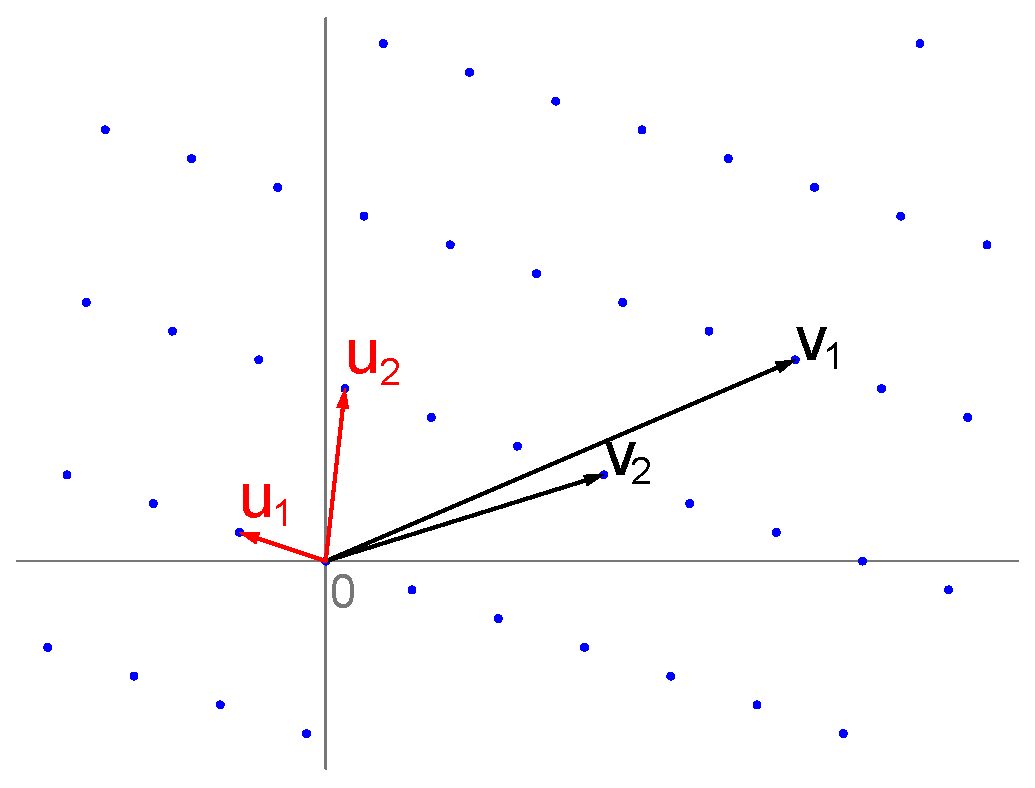
\includegraphics[width=0.8\linewidth]{Lattice-reduction}
  \caption{Two different bases for the same two dimensional lattice.}
  \label{fig:bases}
\end{figure}

\par What we considered earlier were lattices spanned over real $m$-dimensional space $\mathbb{R}^m$ but in similar sense we can consider a lattice consisting of complex valued vectors from $\mathbb{C}^m$. The principles of such complex lattice are almost the same, however, now $\mathbf{B}$ and $\mathbf{a}$ take values from $\mathbb{C}$. Note that a complex lattice has an equivalent real representation which has double the rank of the corresponding complex lattice. Consider a lattice $\Lambda \subset \mathbb{C}^m$ with a generator matrix $\mathbf{B} = [\mathbf{z}_1, ... , \mathbf{z}_n]$. Now we can always express it with a real valued lattice $\Lambda_{\text{real}} \subset \mathbb{R}^{2m}$ and the corresponding $2m \times n$ generator matrix is given by

\begin{equation}
\mathbf{B}_{\text{real}} =
\begin{bmatrix} 
\text{Re}(z_{11}) & \dots  & \text{Re}(z_{1n}) \\
\text{Im}(z_{11}) & \dots  & \text{Im}(z_{1n}) \\
\vdots            & \ddots & \vdots            \\
\text{Re}(z_{m1}) & \dots  & \text{Re}(z_{mn}) \\
\text{Im}(z_{m1}) & \dots  & \text{Im}(z_{mn}) \\
\end{bmatrix}.
\label{eq:complex}
\end{equation}
In other words we convert each column of $\mathbf{B}$ to real vector by separating each of their complex elements into two adjacent real elements, that is the real and imaginary parts of the original complex element. This process doubles the amount of rows in $\mathbf{B}_{\text{real}}$ but both representations ultimately describe the same lattice. \cite{conway}

\subsection{Closest vector problem}

One relevant mathematical problem related to sphere decoding, a communications application of interest in this paper, is the closest vector problem (CVP). Given a lattice $\Lambda \subset J$ and an input point $\mathbf{y} \in J$ the problem is to find a lattice point $\hat{\mathbf{x}} \in \Lambda$ that is closest to $\mathbf{y}$. More precisely $\hat{\mathbf{x}} \in \Lambda$ has to meet the following condition

\begin{equation}
\|\mathbf{y}-\hat{\mathbf{x}}\| \leq \|\mathbf{y}-\mathbf{x}\|, \ \ \ \forall \mathbf{x} \in \Lambda.
\label{eq:cvp}
\end{equation}

\noindent$J$ is the vector space, in which $\Lambda$ belongs in. In this thesis we mostly consider $J=\mathbb{C}^n$. 
\par For a fixed point $\mathbf{x}' \in \Lambda$ the set of vectors $\mathbf{y}_i \in J$ that satisfy the inequality \eqref{eq:cvp} is called the Voronoi region (see figure \ref{fig:voronoi}) of lattice point $\mathbf{x}'$, $\mathcal{V}_{\mathbf{x}'} \subset J$. This means that if $\mathbf{y} \in \mathcal{V}_{\mathbf{x}'}$ then the solution to CVP is $\mathbf{x}'$ as can be clearly seen from figure \ref{fig:voronoi}. If $\mathbf{y} \in \partial\mathcal{V}_{\mathbf{x}'}$ the solution to CVP is a random choice between points whose Voronoi region contains that boundary. The volume of the $\mathcal{V}_{\mathbf{x}'}$, also know as the lattice constant as it is independent of the choice of basis, is given by det$(\Lambda) = $ $\sqrt{\text{det}(\mathbf{B}^T\mathbf{B}})$, where $\mathbf{B}$ is the generator matrix of $\Lambda$. 

\begin{figure}[ht]
% source: http://www.gregegan.net/APPLETS/12/deBruijnNotes.html
  \centering
  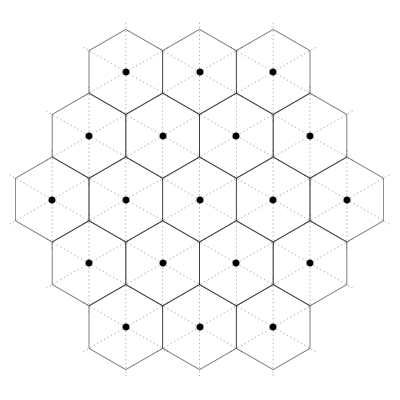
\includegraphics[width=0.5\linewidth]{voronoi_cells}
  \caption{The voronoi cells of the two dimensional hexagonal lattice $\mathsf{A}_2$.}
  \label{fig:voronoi}
\end{figure}

CVP is trivial for orthogonal lattices as one could just round every coordinate of $\mathbf{y}$ to nearest integer an get the correct answer, but CVP has been shown to be NP-hard as the function of the lattice rank in general case when we consider skewed lattices and thus all known algorithms for CVP have exponential worst case complexity \cite{agrell}. Non-trivial lattices appear in most communications applications, for example when using maximum likelihood decoding for a lattice codes sent via channel that induces fading. Such decoding process can be reduced to CVP and it's later explained in further detail.

\subsection{Space--time lattice codes}

Space--time lattice codes are a robust way of encoding the data on a  wireless channel that uses multiple transmit and receiver antennas, i.e. a MIMO-system. Wireless channels are usually very error prone due to interference and fading caused by the surrounding electrical devices, obstacles and nature. This method helps to improve the reliability of the data transmission on such channel, meaning we get decoding errors less likely. A single codeword from certain space--time lattice code constellation can be represented as a matrix that is defined like so

\begin{equation}
\mathcal{L} = \Bigg\{\sum_{i=1}^k a_i\mathbf{X}_i \ \Big| \ \mathbf{X}_i \in \mathcal{M}_{m \times l}(\mathbb{C}), \ a_i \in S \subset \mathbb{Z} \Bigg\}.
\label{eq:codeword}
\end{equation}
The $\mathbf{X}_i, i = 1,...,k$ denote the constant basis matrices of the lattice code and the coefficients $a_i, i = 1,...,k$ are integers from a finite signal set $S$ which represent the data we want to send.



\clearpage

\section{Sphere decoder}

In this chapter we will discuss an efficient decoding algorithm for the space--time block codes known as the sphere decoder. This thesis is particularly interested in the Schnorr-Euchnerr implementation of the algorithm which combines the Pohst strategy and the Babai nearest plane algorithm \cite{agrell}. The problem of decoding the correct codeword from the set of all possible codewords from the received noisy codeword can be reduced to CVP that was discussed earlier. What the sphere decoder basicly does is that instead of searching through all lattice points within the finite signal set boundaries it only considers lattice points within a hypersphere around the received vector of certain radius. This significantly reduces the complexity of the search algorithm. 

\begin{figure}[ht]
% source: http://www.gregegan.net/APPLETS/12/deBruijnNotes.html
  \centering
  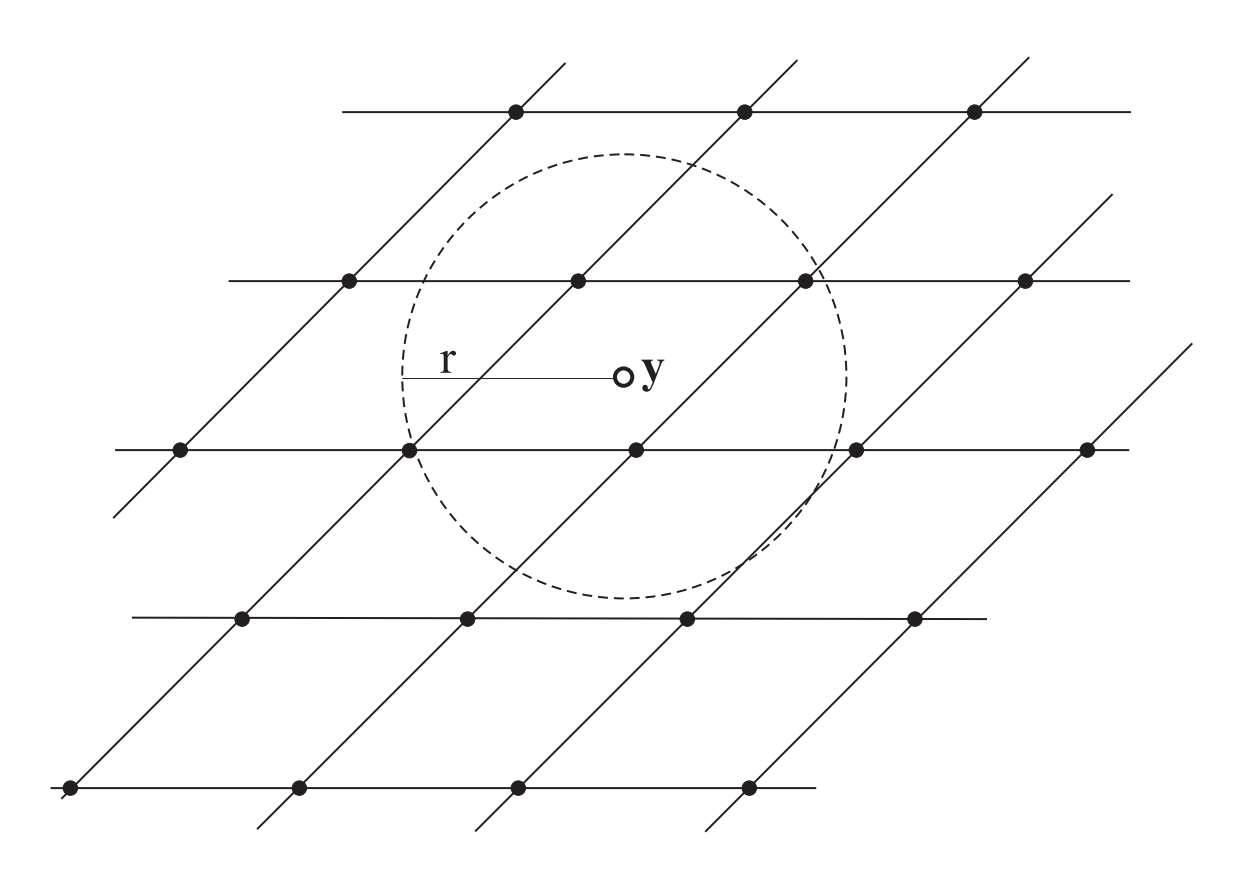
\includegraphics[width=0.8\linewidth]{sphere_decoder}
  \caption{The CVP with sphere decoding in two dimensional lattice. The search complexity can be reduced by giving an upper bound for the closest point distance \cite{mia}.}
  \label{fig:sphdec}
\end{figure}

\par One question remains though, so how do we choose the radius? If it's too small, no lattice points lie within the sphere or if it's too large, the complexity will increase and slow down the algorithm. The answer to that question is, with our Schnorr-Euchnerr implementation of the algorithm, we can simply set it to infinity. It uses by definition the Babai nearest plane algorithm, which requires no upper bound for the distance to the closest point to find a nearby point which we can use to dynamically update the upper bound of the search algorithm to the distance to that point.  Clearly the closest point is either that point we just found, also known as the Babai point, or another one within that radius.

\subsection{Recursive sublattice decomposition}

For understanding how the sphere decoder works we introduce the concept of sublattice decomposition from $n$-dimensional lattice to a stack of $(n-1)$-dimensional sublattices. As one could guess this can also be done recursively and ultimately we end up with 0-dimensional lattices also known as the lattice points. The motivation to this recursive representation of a lattice is that one only needs to consider intervals of sublattice layer indices when doing the distance comparison in each dimension from $n$ to $0$.
\par Let us consider a $m \times n$ lattice generator matrix $\mathbf{G}$ for a lattice $\Lambda$ and write it like
 
\begin{equation}
\mathbf{G} = \big[\mathbf{G}' \ \ \mathbf{v}_n \big]
\label{eq:gen}
\end{equation}
where $\mathbf{G}'$ is a $m \times (n-1)$ matrix and the last column vector can be written as $\mathbf{v}_n = \mathbf{v}_{\parallel} + \mathbf{v}_{\bot}$, with $\mathbf{v}_{\parallel}$ in the column space of $\mathbf{G}'$ and $\mathbf{v}_{\bot}$ in the null space of $\mathbf{G}'$. With this notation we can decompose any $n$-dimensional lattice as follows

\begin{equation}
\Lambda(\mathbf{G}) = \bigcup_{u_n=-\infty}^{+\infty} \big\{\mathbf{c}+u_n\mathbf{v}_{\parallel}+u_n\mathbf{v}_{\bot} \mid \mathbf{c} \in \Lambda(\mathbf{G}') \big\}.
\label{eq:decom}
\end{equation}

\noindent Equation \eqref{eq:gen} basically describes a stack of $(n-1)$-dimensional translated sublattices, where $u_n$ is the index of each sublattice of an $n$-dimensional lattice $\Lambda$. The hyperplanes over which the sublattices are spanned are called \textit{layers}. For example you can think of the horizontal lines in figure \ref{fig:sphdec} as one dimensional layers and the discrete points in them as a sublattice of the whole two dimensional lattice. 
\par To better understand the the given expression in equation \eqref{eq:gen} let's consider the sublattice in the base layer $u_n = 0$, which is just all the points in the sublattice generated by $\mathbf{G}'$. Similarly we can get all other sublattices from this base sublattice by offsetting all the points in it by linear combination $u_n\mathbf{v}_{\parallel}+u_n\mathbf{v}_{\bot}$, where $\mathbf{v}_{\parallel}$ denotes a translation of all points in that same hyperplane and $\|\mathbf{v}_{\bot}\|$ is the orthogonal distance between two adjacent layers in the $n$th dimension. By taking the union of all these sublattices we get the whole $n$-dimensional lattice. In figure \ref{fig:sphdec} for example you can think of the middle horizontal line as the base layer.
\par If $\mathbf{G}$ is an upper triangular matrix, we can easily express $\mathbf{v}_{\bot}$ as $\mathbf{v}_{\bot} = (0, 0, ..., v_{nn})^T$ and thus we can write simply $\|\mathbf{v}_{\bot}\| = |v_{nn}|$. In fact any generator matrix $\mathbf{G}$ can be rotated to upper triangular form \cite{agrell} with $v_{nn} > 0$ so we can simply denote the distance between $(k-1)$-dimensional layers with $v_{kk}$ later on.
\par With the consept of recursive sublattice decomposition a search algorithm in $n$-dimensional lattice $\Lambda(\mathbf{G})$ can be described recursively as a finite number of ($n-1$)-dimensional search operations. If $\mathbf{x} \in \mathbb{R}^m$ is a vector to decode in the lattice $\Lambda(\mathbf{G})$, which is decomposed as in \eqref{eq:decom}, the orthogonal distance from $\mathbf{x}$ to the layer with index $u_n$ is given by the formula
\begin{equation}
y_n = |u_n-\hat{u}_n| \cdot \|\mathbf{v}_{\bot}\|
\label{eq:dist}
\end{equation}
where
\begin{equation}
\hat{u}_n = \frac{\mathbf{xv}_{\bot}^t}{\|\mathbf{v}_{\bot}\|^2}
\label{eq:uhat}
\end{equation}
\clearpage

\section{Simulations and results}
 
\clearpage

\section{Summary}


\clearpage
%% The \phantomsection command is nessesary for hyperref to jump to the 
%% correct page, in other words it puts a hyper marker on the page.

\phantomsection
\addcontentsline{toc}{section}{\refname}
%\addcontentsline{toc}{section}{References}
\begin{thebibliography}{99}

\bibitem{mia} Mäki,\ M. \textit{Space-time block codes and the complexity of sphere decoding.} Doria, Referenced 10.7.2017. Available:
  \url{https://www.doria.fi/bitstream/handle/10024/54404/gradu2008maki-miia.pdf}
  
  
\bibitem{cassels} Cassels, J.W.S. \textit{An introduction to the Geometry of Numbers}, New York, Springer--Verlag, 1971.

\bibitem{agrell} Agrell, E., Eriksson, T. and Zeger, K. \textit{Closest point search in lattices} IEEE Transactions on Information Theory, Vol. 48, pp.2201-2214,
August 2002.

\bibitem{conway} Conway,\ J.H. and Sloane,\ N.J.A. \textit{Sphere packings, lattices and groups.} Third edition, New York, Springer--Verlag, 1998.


\end{thebibliography}

%% Appendices
%% Liitteet
\clearpage

\thesisappendix

\section{Program User Guide}

\subsection{Abbreviations}
\begin{tabular}{ll}
SNR & Signal to noise ratio \\
CPU & Central processing unit \\
RAM & Random access memory \\
GPU & Graphical processing unit \\
C++ & C++ programming language \\
OS & Operating system \\
\end{tabular}

\subsection{Preface}
The purpose of this program is to simulate the performance of different space--time lattice codes under different levels of SNR. It is a command line application that uses simple text based files for input and output. It also has a optional plotting utility which provides graphical interface for the simulation results. The program is primalily intented to be used on Linux based operating systems but should be portable to other platforms as well (there are some slight differences in the required compiler instructions and used libraries though). This guide assumes Linux based operating system, the steps described here might differ slightly when the program is used on other operating systems. The details regarding to those differences are not discussed here. In the following chapters we will go through the installation and usage of the program in detail. 

\subsection{System requirements}

Regarding the hardware as the rule of the thumb, the better the performance your computer has the faster the simulations, although nearly all modern computers with a keyboard and a monitor should suffice for small simulations. The program makes use of parallel CPU cores so one does not need to worry too much about single thread performance of the CPU. The program should not be too memory consuming except in some special use cases so no excessive amount of RAM is needed for fast simulations. GPU support might also be implemented in the future but for now the choice of GPU is irrelevant regarding the simulations.
\par Before trying to install and run the program itself, you need to make sure you have the all the required libraries and a compatible C++ compiler installed. The recommended GNU C++ compiler (g++) should be preinstalled in most Linux distributions but in case it is not, please refer to installation notes here: \url{https://gcc.gnu.org/wiki/InstallingGCC}. 
\par The next thing is to gather the required library packages:
\begin{enumerate}
\item OpenBLAS library: \url{https://github.com/xianyi/OpenBLAS/wiki/Installation-Guide}
\item LAPACK -- Linear Algebra PACKage: \url{http://www.netlib.org/lapack}
\item ARPACK library: \url{http://www.caam.rice.edu/software/ARPACK}
\item Armadillo C++ Linear algebra library: \url{http://arma.sourceforge.net/download.html} 
\item Boost C++ library (optional, for plotting only): \url{http://www.boost.org}
\end{enumerate}
% (libarmadillo-dev)
You can follow the links for detailed instructions on how install those packages if you're facing problems (e.g. you're not installing the program on Linux OS) but the most straightforward way of doing this is by opening a terminal in Linux (CTRL+ALT+T) and using the package manager utility (e.g. apt-get in Ubuntu) to install those packages. The first three packages are required by the Armadillo library so you should install the packeges in the given order. Also note that not Linux based operating systems might require different libraries for Armadillo to work, in this case please refer to the Armadillo documentation by following the given link. 
\par In the Linux package manager the libraries listed should go by names: \textit{libopenblas-dev}, \textit{liblapack-dev}, \textit{libarpack-dev}, \textit{libarmadillo-dev} and \textit{libboost-all-dev}. Note that there might be some version number before the first dash in those names. The Boost library can safely be omitted for compability reasons, but requires a few modifications in the source code and Makefile for the compilation process. If all the install processes succeed you are now all set up to install the program itself.

\subsection{Installing the program}

Open terminal (CTRL+ALT+T) and create a folder for the program 
\begin{verbatim}
$ mkdir sphere-decoder
$ cd sphere-decoder
\end{verbatim}Once you are in that folder copy the contents of this Gitlab repository there: \url{https://version.aalto.fi/gitlab/pasi.pyrro/sphere-decoder}. This can be done by either downloading the repository as a compressed folder (e.g. zip) and extracting it into the folder created earlier or by using the following command in the terminal:
\begin{verbatim}
$ git clone git@version.aalto.fi:pasi.pyrro/sphere-decoder.git
\end{verbatim}

\noindent After copying the files check the contents of that folder by typing this command in the terminal:
\begin{verbatim}
$ ll
\end{verbatim}
Check if the contents of that folder look similar to those of the gitlab repository. If everything looks all right and you're using Linux with Boost library, just type the following in terminal
\begin{verbatim}
$ make
\end{verbatim}
to compile the program. For other operating systems you likely need to modify the Makefile located in the /src/ directory. If you didn't install the Boost C++ library you need to do the following in order to compile the program:
\begin{verbatim}
$ nano src/misc.hpp
\end{verbatim}
In the text editor locate a line of code saying
\begin{verbatim}
#define PLOTTING // enable plotting (requires boost C++ library)
\end{verbatim}
and either remove it or comment it out (type '//' in front of the line). After that save and exit by pressing CTRL+O, ENTER and CTRL+X. After that type the command:
\begin{verbatim}
$ nano src/Makefile
\end{verbatim}
and remove all the compiler flags that have the word 'lboost' in it. Save changes and exit the text editor as before. Now you should be able to compile the program by typing:
\begin{verbatim}
$ make
\end{verbatim}

\noindent If the compiling succeeded, now check if the program runs correctly by typing:
\begin{verbatim}
$ make run
\end{verbatim}
If there are no errors regarding missing libraries or such then you have just correctly installed the program! If there are such errors during the compilation or program runtime, go back to previous section and double check that you have installed the correct libraries. 

\subsection{Setup and Input}

Now that the program runs it is time to take a look at the simulation parameters and the program input to make reasonable simulations. In the /bases/ folder one can save text files containing the lattice code basis matrices for the simulation which the program takes as input. The basis file for the Alamouti code should already be there and is used as the default. When creating a new basis file, one should stick to either Mathematica or Matlab syntax for complex matrices to ensure correct interpretation of the input. 
\par For simulation parameters and other options one should navigate to /settings/ folder and open the default settings file called \textit{settings.ini}. The contents of the file are displayed in figure \ref{fig:settings}. After '//' begins a comment sequence which is ignored by the program when reading the settings file. Make sure not to remove any of the 15 option lines or the program will give you an error. In case you end up messing up the settings file in some way, easy way to reset it is to just delete it and run the program normally. This will generate a new default settings file for you, like the one in figure \ref{fig:settings}.

\begin{figure}[htb]
\begin{center}
  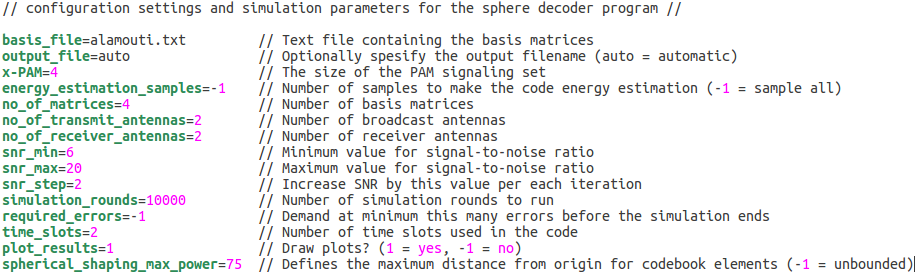
\includegraphics[width=\linewidth]{settings}
  \caption{The default settings file for the sphere decoder program.}
  \label{fig:settings}
\end{center}
\end{figure}

When editing the settings, only modify the right hand side of the equality sign. If you change the variable names, the program will work incorrectly. You can always check the correct variable names from figure \ref{fig:settings} or just generate a new default settings file if you happen to change them accidentally. Another rule of the thumb is that if you want to use default behaviour for some feature, use -1 value for that variable. The order of the setting variables does not matter, just make sure they're all on their own separate line. Remember to save the changes you make to that file. The program doesn't need to be recompiled for these changes to take effect, just run it again. 
\par One can also create multiple settings file in that folder. To use a different settings file one just needs to give its name as a command line argument for the program.

\subsection{Running the program}

Once the program is set up correctly, running the program is a relatively easy task. Just make sure you're in the main folder of the local repository and type the following in terminal:
\begin{verbatim}
$ make run
\end{verbatim}
or
\begin{verbatim}
$ ./sphdec [settings_file.ini*]
\end{verbatim}

\noindent The first command uses the default settings file and in the second one can optionally spesify the name of the settings file to be used (do not give the whole file path, just the name of a file in /settings/ folder). If no command line argument is given the two commands are equal.
\par Once the program has started it prints useful data related to the current actions it is taking to the terminal as well as in the log.txt file located in the /logs/ folder. Visiting the log.txt file can be useful for reviewing previous program behaviour in the future. In the log file each program runtime should be separated by an empty line.
\par If the program gets stuck somewhere or takes too long to finish a large simulation, pressing CTRL+C in the terminal will terminate the execution of the program instantly. Although doing this may result in a loss of data calculated so far. For large simulations one needs to be patient as the simulation complexity is NP-hard as the function of lattice code dimension.

\subsection{Output and Plots}

If the program exits without errors its output should be found from /output/ folder in csv format. The filenames are by default named so that they are in chronological order so the latest simulation output should be the last one in the file listing. The csv format is easy to import in other programs like Matlab.
\par If the program was compiled successfully with the PLOTTING flag enabled and the following settings variable is set to
\begin{verbatim}
plot_results=1 
\end{verbatim}
then a couple of graphical interfaces for plots generated from the simulation data should pop up. If there are errors check that you also have GNUPlot installed on your system. Plotting gives you a quick review on how the simulation went. For more rigorous data analysis it is recommended to import the output csv file to some numerical scientific calculation software like Matlab.

\subsection{General troubleshooting}
Some general miscellaneous tips are listed here to help you troubleshoot errors while using the program:
\begin{enumerate}
\item Do not include the dollar sign in terminal commands. It's just there to indicate terminal input.
\end{enumerate}


\end{document}
